\documentclass[tikz,border=3pt]{standalone}
\usepackage{tikz}

\begin{document}
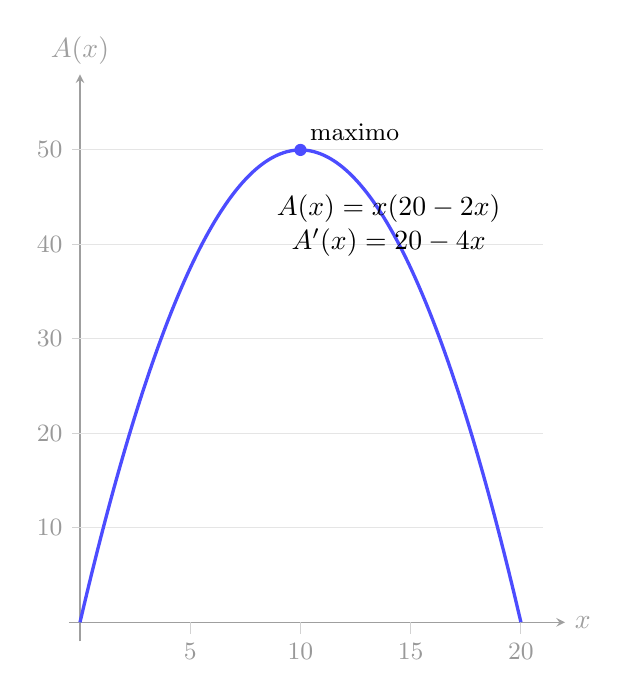
\begin{tikzpicture}[x=0.28cm,y=0.12cm,>=stealth]
  \draw[->,gray!75] (-0.5,0) -- (22,0) node[right] {$x$};
  \draw[->,gray!75] (0,-2) -- (0,58) node[above] {$A(x)$};

  \foreach \x in {5,10,15,20} {
    \draw[gray!35] (\x,0) -- (\x,-1.2) node[below,gray!80] {\small \x};
  }
  \foreach \y in {10,20,30,40,50} {
    \draw[gray!20] (0,\y) -- (21,\y);
    \draw[gray!35] (0,\y) -- (-0.35,\y) node[left,gray!80] {\small \y};
  }

  \draw[domain=0:10,samples=80,smooth,very thick,blue!70]
    plot ({2*\x},{\x*(20-2*\x)});
  \fill[blue!70] (10,50) circle (2.2pt)
    node[above right,black] {\small maximo};

  \node[align=center,black] at (14,42)
    {$A(x)=x(20-2x)$\\$A'(x)=20-4x$};
\end{tikzpicture}
\end{document}
